
\subsection{Part 1}

In this part we begin by comparing the expected and observed wavelengths and energies of the spectral lines of the hydrogen atom. The expected wavelengths and energies are calculated using the Rydberg formula, and the observed values are obtained from the spectrometer. The results are shown in Table \ref{tab:Part1_expected_vs_observed} and the plots in Figures \ref{fig:Part1wave} and \ref{fig:Part1energy}.
The residuals are shown in Figures \ref{fig:Part1waveU} and \ref{fig:Part1energyU} respectively.

The observed wavelengths and energies to do not fall within the uncertainty range of the real values, however, most of the values do fit within 2 uncertainty intervals. There seem to be a fixed offset between the real and observed values. This can be also also seen in the linear fit equations in figures \ref{fig:Part1wave} and \ref{fig:Part1energy}.
This could indicate that the spectrometer is not properly calibrated.

\begin{table}
    \begin{adjustbox}{width=1.5\textwidth, center}
        \begin{tabular}{|c|c|c|c|c|c|c|}
            \hline Color              & Violet            & Violet            & Blue              & Green             & Yellow            & Yellow        \\
            \hline \begin{tabular}{c}
                       Expected $\lambda$, \\
                       $\mathrm{nm}$
                   \end{tabular} & 404.6565          & 407.7837          & 435.8328          & 546.0735          & 576.9598          & 579.0663           \\
            \hline \begin{tabular}{c}
                       Expected energies, \\
                       $\mathrm{eV}$
                   \end{tabular} & 3.064             & 3.040             & 2.845             & 2.270             & 2.149             & 2.141              \\
            \hline \begin{tabular}{c}
                       Experiment $\lambda$, \\
                       $\mathrm{nm}$
                   \end{tabular} & 409.40 $\pm$ 3.58 & 412.60 $\pm$ 3.58 & 439.00 $\pm$ 3.58 & 541.40 $\pm$ 4.48 & 570.90 $\pm$ 6.27 & 573.30  $\pm$ 6.27 \\
            \hline \begin{tabular}{c}
                       Experiment energy, \\
                       $\mathrm{eV}$
                   \end{tabular} & 3.03$\pm$0.03     & 3.00$\pm$0.03     & 2.82$\pm$0.02     & 2.29$\pm$0.02     & 2.17$\pm$0.02     & 2.16$\pm$0.02      \\
            \hline
        \end{tabular}
    \end{adjustbox}
    \caption{Observed and expected wavelengths and energies of the spectral lines of the hydrogen atom.}
    \label{tab:Part1_expected_vs_observed}

\end{table}

\subsubsection{Expected vs observed wavelengths}

The best line fit for the expected vs observed wavelengths is given by equation \ref{eq:Part1wave}, where $\lambda_{\text {exp }}$ is the observed wavelength and $\lambda_{\text {th }}$ is the expected wavelength.

\begin{equation}
    \lambda_{\text {exp }} = (0.839 \pm 0.002) \lambda_{\text {th }} + (27.508 \pm 0.9) \text{nm}
    \label{eq:Part1wave}
\end{equation}

The residuals plot can be seen in Figure \ref{fig:Part1waveU}. The residuals seem to exhibit a random pattern, which is a indication that the fit is good. At each point, the line of best fit is within
the uncertainty range of the observed value.

\begin{equation}
    \chi^2 = 1.088 \qquad
    \frac{\chi^2}{v} = 0.272
\end{equation}

% Add plots and residuals
\begin{figure}[H]
    \centering
    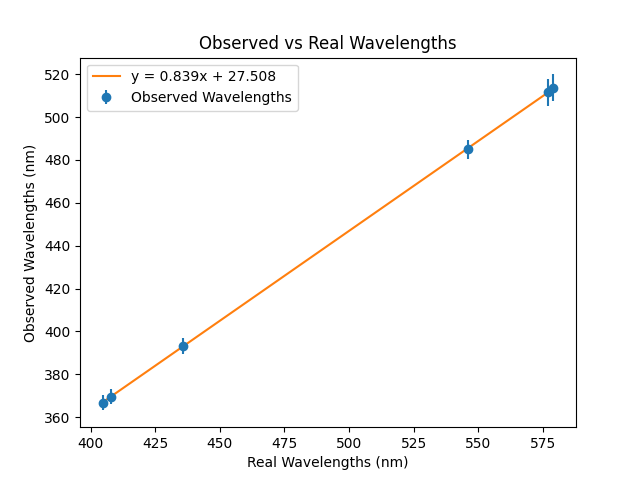
\includegraphics[width=0.8\textwidth]{Results/Sections/Part1/Part1_wavelength_observed_vs_expected.png}
    \caption{Observed vs expected wavelengths}
    \label{fig:Part1wave}
\end{figure}


\begin{figure}[H]
    \centering
    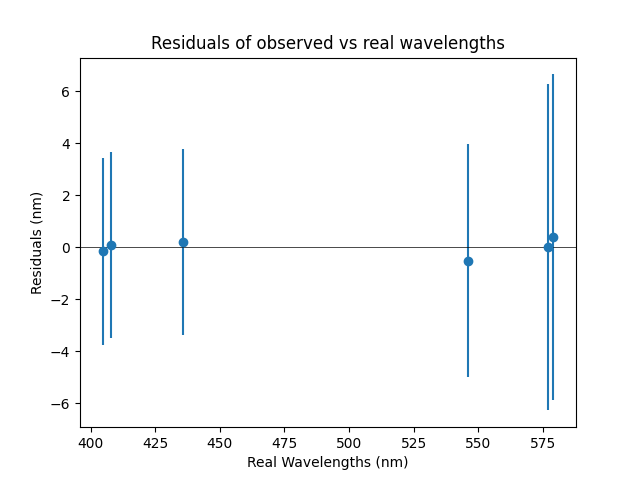
\includegraphics[width=0.8\textwidth]{Results/Sections/Part1/Part1_wavelength_observed_vs_expected_residuals.png}
    \caption{Observed vs expected wavelengths residuals}
    \label{fig:Part1waveU}
\end{figure}



\subsubsection{Expected vs observed energies}

The best line fit for the expected vs observed wavelengths is given by equation \ref{eq:Part1eng}, where $E_{\text {exp }}$ is the observed wavelength and $E_{\text {th }}$ is the expected wavelength.

\begin{equation}
    E_{\text {exp }} = (1.0439 \pm 0.003) E_{\text {th }} + (0.1818 \pm 0.007) \text{eV}
    \label{eq:Part1eng}
\end{equation}

The residuals plot can be seen in Figure \ref{fig:Part1waveU}. Again, the residuals seem to exhibit a random pattern, which is a indication that the fit is good. At each point, the line of best fit is within
the uncertainty range of the observed value.

\begin{equation}
    \chi^2 = 1.103 \qquad
    \frac{\chi^2}{v} = 0.275
\end{equation}


\begin{figure}[H]
    \centering
    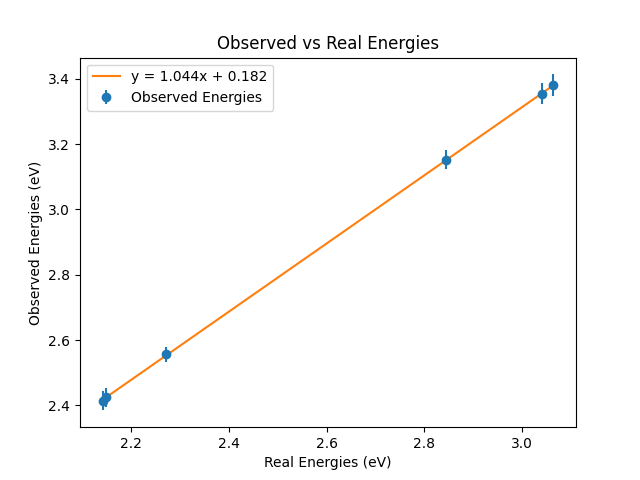
\includegraphics[width=0.8\textwidth]{Results/Sections/Part1/Part1_energy_observed_vs_expected.png}
    \caption{Observed vs expected energies}
    \label{fig:Part1energy}
\end{figure}

\begin{figure}
    \centering
    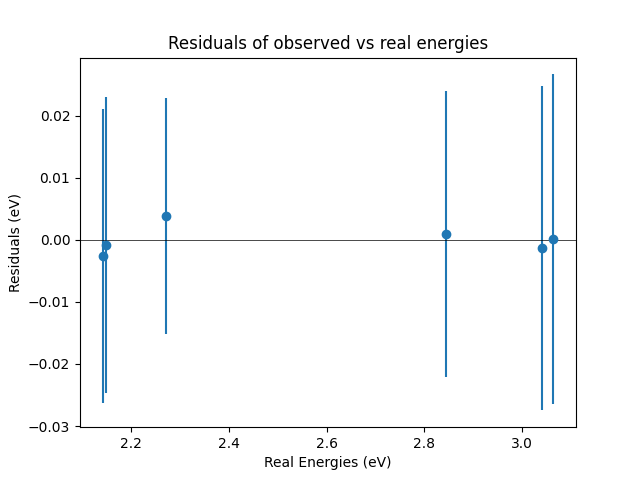
\includegraphics[width=0.8\textwidth]{Results/Sections/Part1/Part1_energy_observed_vs_expected_residuals.png}
    \caption{Observed vs expected energies residuals}
    \label{fig:Part1energyU}
\end{figure}



% line: 0.8387695642338823 ± 0.001864112875415517 x + 27.508082396595857 ± 0.9278156049052266
% Chi squared: 1.087797528170102
% Reduced chi squared: 0.2719493820425255

% line: 1.0439270677118886 ± 0.0028012430069567747 x + 0.18182109169387295 ± 0.007329939614454457
% Chi squared: 1.1027736664663765
% Reduced chi squared: 0.27569341661659413